%!TEX root=../main.tex
% Chapter Template

\chapter{Implementation} % Main chapter title

\label{Chapter5} % Change X to a consecutive number; for referencing this chapter elsewhere, use \ref{ChapterX}

%----------------------------------------------------------------------------------------
%	SECTION 1
%----------------------------------------------------------------------------------------

\section{Solution overview}

The final solution consists of a \gls{REST} API build with ASP.NET Core and a MongoDB \gls{NoSQL} database. Both are hosted through Amazon Webservices in an EC2 container using Docker. \\
The API consists of the commands seen in appendix \ref{APICommands}. \\\\

This section covers the process from the initial data delivery to the final solution in a chronological order.

\section{Initial data dump}
In the beginning of the project we were supplied with data from one of \gls{Struct} customers. This data was in the form of many SQL tables and most of the data was not relevant for creating product recommendations. The main tables used were the following:  \\
\begin{itemize}
\item Visitor: A collection of every unique visitor who visited the customer's website, each visitor gets a unique identifier called UID. Contains 3,073,665  visitors.
\item Profile: A collection of every users signed up at the website. Contains 3037 profiles.
\item BehaviorData: A collection of every unique action performed by visitors on the website, for example when a visitor views a product a new row is made with the visitor's UID, the product UID and the timestamp. Contains 3,326,736 visitor actions.
\item Order: Contains each profile's orders. Contains 5520 orders.
\end{itemize}

A snapshot of the visitor and behaviorData table can be seen in figure \ref{visitorTable} and \ref{behaviorTable}.

\begin{figure}[H]
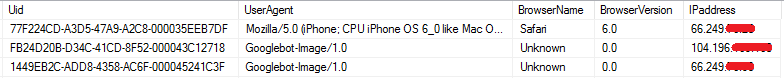
\includegraphics[scale=0.8]{Visitor_table}
\caption{Visitor table from the original data}
\label{visitorTable}
\end{figure}
\begin{figure}[H]
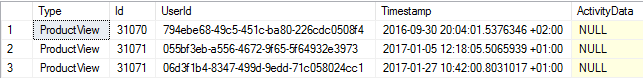
\includegraphics{behaviorData_table}
\caption{Behavior data table from the original data}
\label{behaviorTable}
\end{figure}

These tables contain all the pertinent information for creating product recommendations and can be utilized after a cleaning and structuring process. This process is described in the following sections.

\section{Data Transformation}
To begin the initial data transformation a data storing technology has to be selected. The technology chosen was \gls{NoSQL}, specifically \gls{MongoDB} the most popular No-SQL framework \cite{DBRankings}. \\
\gls{NoSQL} is chosen because of the good fit for this project. The data demands are not clearly specified in the beginning and with No-SQL it is easy to add or remove data or even change the data types on the fly. No-SQL's denormalized format also allows for faster retrieval of a single item without having to do joins or complex SQL queries. Finally No-SQL is easier to scale across multiple servers and many engines have built in scaling functionalities \cite{SQLvsNOSQL} which can come in handy when multiple clients begin using the service. \\\\

A brief overview of the different terminology for SQL and No-SQL is given in table \ref{sqlvsnosql_table}.
\begin{table}[H]
\centering
\caption{SQL vs No-SQL terminology}
\label{sqlvsnosql_table}
\begin{tabular}{|l|l|p{8cm}|}
\hline
\textbf{SQL}   & \textbf{No-SQL}     & \textbf{Comment}                                                                                                    \\ \hline
Table & Collection &                                                                                                            \\ \hline
Row   & Document   & A No-SQL document can contain more complex datatype compared to a row in SQL e.g arrays or other documents \\
\hline
\end{tabular}
\end{table}

Python was used to accomplish the early migration from SQL tables to MongoDB.  